\documentclass[]{article}
\usepackage{lmodern}
\usepackage{amssymb,amsmath}
\usepackage{ifxetex,ifluatex}
\usepackage{fixltx2e} % provides \textsubscript
\ifnum 0\ifxetex 1\fi\ifluatex 1\fi=0 % if pdftex
  \usepackage[T1]{fontenc}
  \usepackage[utf8]{inputenc}
\else % if luatex or xelatex
  \ifxetex
    \usepackage{mathspec}
  \else
    \usepackage{fontspec}
  \fi
  \defaultfontfeatures{Ligatures=TeX,Scale=MatchLowercase}
\fi
% use upquote if available, for straight quotes in verbatim environments
\IfFileExists{upquote.sty}{\usepackage{upquote}}{}
% use microtype if available
\IfFileExists{microtype.sty}{%
\usepackage{microtype}
\UseMicrotypeSet[protrusion]{basicmath} % disable protrusion for tt fonts
}{}
\usepackage[margin=1in]{geometry}
\usepackage{hyperref}
\hypersetup{unicode=true,
            pdfborder={0 0 0},
            breaklinks=true}
\urlstyle{same}  % don't use monospace font for urls
\usepackage{color}
\usepackage{fancyvrb}
\newcommand{\VerbBar}{|}
\newcommand{\VERB}{\Verb[commandchars=\\\{\}]}
\DefineVerbatimEnvironment{Highlighting}{Verbatim}{commandchars=\\\{\}}
% Add ',fontsize=\small' for more characters per line
\usepackage{framed}
\definecolor{shadecolor}{RGB}{248,248,248}
\newenvironment{Shaded}{\begin{snugshade}}{\end{snugshade}}
\newcommand{\KeywordTok}[1]{\textcolor[rgb]{0.13,0.29,0.53}{\textbf{{#1}}}}
\newcommand{\DataTypeTok}[1]{\textcolor[rgb]{0.13,0.29,0.53}{{#1}}}
\newcommand{\DecValTok}[1]{\textcolor[rgb]{0.00,0.00,0.81}{{#1}}}
\newcommand{\BaseNTok}[1]{\textcolor[rgb]{0.00,0.00,0.81}{{#1}}}
\newcommand{\FloatTok}[1]{\textcolor[rgb]{0.00,0.00,0.81}{{#1}}}
\newcommand{\ConstantTok}[1]{\textcolor[rgb]{0.00,0.00,0.00}{{#1}}}
\newcommand{\CharTok}[1]{\textcolor[rgb]{0.31,0.60,0.02}{{#1}}}
\newcommand{\SpecialCharTok}[1]{\textcolor[rgb]{0.00,0.00,0.00}{{#1}}}
\newcommand{\StringTok}[1]{\textcolor[rgb]{0.31,0.60,0.02}{{#1}}}
\newcommand{\VerbatimStringTok}[1]{\textcolor[rgb]{0.31,0.60,0.02}{{#1}}}
\newcommand{\SpecialStringTok}[1]{\textcolor[rgb]{0.31,0.60,0.02}{{#1}}}
\newcommand{\ImportTok}[1]{{#1}}
\newcommand{\CommentTok}[1]{\textcolor[rgb]{0.56,0.35,0.01}{\textit{{#1}}}}
\newcommand{\DocumentationTok}[1]{\textcolor[rgb]{0.56,0.35,0.01}{\textbf{\textit{{#1}}}}}
\newcommand{\AnnotationTok}[1]{\textcolor[rgb]{0.56,0.35,0.01}{\textbf{\textit{{#1}}}}}
\newcommand{\CommentVarTok}[1]{\textcolor[rgb]{0.56,0.35,0.01}{\textbf{\textit{{#1}}}}}
\newcommand{\OtherTok}[1]{\textcolor[rgb]{0.56,0.35,0.01}{{#1}}}
\newcommand{\FunctionTok}[1]{\textcolor[rgb]{0.00,0.00,0.00}{{#1}}}
\newcommand{\VariableTok}[1]{\textcolor[rgb]{0.00,0.00,0.00}{{#1}}}
\newcommand{\ControlFlowTok}[1]{\textcolor[rgb]{0.13,0.29,0.53}{\textbf{{#1}}}}
\newcommand{\OperatorTok}[1]{\textcolor[rgb]{0.81,0.36,0.00}{\textbf{{#1}}}}
\newcommand{\BuiltInTok}[1]{{#1}}
\newcommand{\ExtensionTok}[1]{{#1}}
\newcommand{\PreprocessorTok}[1]{\textcolor[rgb]{0.56,0.35,0.01}{\textit{{#1}}}}
\newcommand{\AttributeTok}[1]{\textcolor[rgb]{0.77,0.63,0.00}{{#1}}}
\newcommand{\RegionMarkerTok}[1]{{#1}}
\newcommand{\InformationTok}[1]{\textcolor[rgb]{0.56,0.35,0.01}{\textbf{\textit{{#1}}}}}
\newcommand{\WarningTok}[1]{\textcolor[rgb]{0.56,0.35,0.01}{\textbf{\textit{{#1}}}}}
\newcommand{\AlertTok}[1]{\textcolor[rgb]{0.94,0.16,0.16}{{#1}}}
\newcommand{\ErrorTok}[1]{\textcolor[rgb]{0.64,0.00,0.00}{\textbf{{#1}}}}
\newcommand{\NormalTok}[1]{{#1}}
\usepackage{longtable,booktabs}
\usepackage{graphicx,grffile}
\makeatletter
\def\maxwidth{\ifdim\Gin@nat@width>\linewidth\linewidth\else\Gin@nat@width\fi}
\def\maxheight{\ifdim\Gin@nat@height>\textheight\textheight\else\Gin@nat@height\fi}
\makeatother
% Scale images if necessary, so that they will not overflow the page
% margins by default, and it is still possible to overwrite the defaults
% using explicit options in \includegraphics[width, height, ...]{}
\setkeys{Gin}{width=\maxwidth,height=\maxheight,keepaspectratio}
\IfFileExists{parskip.sty}{%
\usepackage{parskip}
}{% else
\setlength{\parindent}{0pt}
\setlength{\parskip}{6pt plus 2pt minus 1pt}
}
\setlength{\emergencystretch}{3em}  % prevent overfull lines
\providecommand{\tightlist}{%
  \setlength{\itemsep}{0pt}\setlength{\parskip}{0pt}}
\setcounter{secnumdepth}{0}
% Redefines (sub)paragraphs to behave more like sections
\ifx\paragraph\undefined\else
\let\oldparagraph\paragraph
\renewcommand{\paragraph}[1]{\oldparagraph{#1}\mbox{}}
\fi
\ifx\subparagraph\undefined\else
\let\oldsubparagraph\subparagraph
\renewcommand{\subparagraph}[1]{\oldsubparagraph{#1}\mbox{}}
\fi

%%% Use protect on footnotes to avoid problems with footnotes in titles
\let\rmarkdownfootnote\footnote%
\def\footnote{\protect\rmarkdownfootnote}

%%% Change title format to be more compact
\usepackage{titling}

% Create subtitle command for use in maketitle
\newcommand{\subtitle}[1]{
  \posttitle{
    \begin{center}\large#1\end{center}
    }
}

\setlength{\droptitle}{-2em}

  \title{}
    \pretitle{\vspace{\droptitle}}
  \posttitle{}
    \author{}
    \preauthor{}\postauthor{}
    \date{}
    \predate{}\postdate{}
  
\usepackage{graphicx,latexsym}
\usepackage{amssymb,amsthm,amsmath}
\usepackage{longtable,booktabs,setspace}

\begin{document}

\section{Orthocore: herramienta para encontrar el core conservado en un
linaje
genómico.}\label{orthocore-herramienta-para-encontrar-el-core-conservado-en-un-linaje-genomico.}

\begin{figure}[h!tbp]
\centering
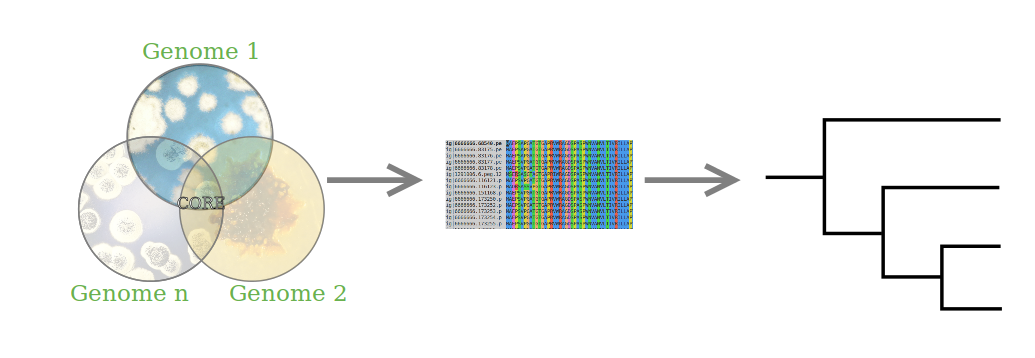
\includegraphics[angle = 0,scale = 1]{chapter1/coreWiki.png}
\caption[coreWiki]{\normalsize{coreWiki}}
\label{fig:coreWiki}
\end{figure}

El pangenoma es el contenido génico total de un linaje taxonómico. Las
familias génicas del pangenoma pueden clasificarse según sus patrones de
presencia y ausencia en cada genoma del linaje. De acuerdo a esta
clasificación los principales grupos de familias génicas en un pangenoma
son el \emph{core}, el \emph{shell} y el \emph{cloud (dispensable)
genome}. El \emph{core genome} es el conjunto de familias con presencia
en todos los genomas del linaje. El \emph{shell genome} es el grupo de
familias presentes en la mayoría de los genomas, mientras que el
\emph{cloud genome} o \emph{dispensable genome} es aquel grupo de
familias que sólo ocurre en unos cuantos genomas.

Orthocore es un desarrollo bioinformático que realicé para calcular las
familias génicas más conservadas del core genome. Orthocore obtiene el
core conservado es decir familias de ortólogos presentes en todos los
genomas del grupo, libres de parálogos e independientes de un genoma de
referencia.

Los cambios en los perfiles de promiscuidad aparece en copias extras de
familias de ortólogos y debido a la pérdida y ganancia de genes en
organismos cercanos, se necesita un algoritmo para poder organizar
filogenéticamente un organismo.

\subsection{El core genome permite la obtención de filogenias
complicadas}\label{el-core-genome-permite-la-obtencion-de-filogenias-complicadas}

Dos secuencias son homólogas si poseen un ancestro común. Ortólogos y
parálogos constituyen los dos principales tipos de homólogos. Los
ortólogos provienen de eventos de especiación de un ancestro común
mientras que los parálogos evolucionan por eventos de duplicación. La
comparación de la variación molecular entre ortólogos ha sido utilizada
para establecer relaciones filogenéticas entre organismos. Por ejemplo
comparar la secuencia de 16s de RNA ribosomal condujo al descubrimiento
del dominio Archaea en 1977 {[}@woese\_phylogenetic\_1977{]}.

Los dos factores importantes para establecer las relaciones
filogenéticas diferenciando entre Archaea, Bacteria y Eucarya son los
siguientes: 1) la presencia conservada de la unidad de 16s en los tres
dominios mencionados, y 2) la suficiente divergencia entre estas
secuencias en organismos de estos dominios. Ahora bien, establecer
relaciones filogenéticas entre Archaea y Bacteria es más sencillo que
establecerlas entre organismos pertenecientes al mismo género o
inclusive a la misma especie. En ocasiones como en el caso del género
\emph{Streptomyces} la secuencia de 16s por sí sola no posee la
suficiente variación para resolver la filogenia
{[}@labeda\_phylogenetic\_2017{]} ya que la variación entre estas
secuencias suele ser menor al 1\%.

Para resolver el problema de escasa variación en secuencias de 16s se
puede concatenar la información de otros ortólogos, siempre que estos
aparezcan en todos los organismos que se estén estudiando, es decir
siempre que sean parte del core genómico. Los ortólogos suelen buscarse
por similitud de secuencia, pero estos métodos suelen también capturar
parálogos, que pueden confundir la elucidación de eventos de
especiación.

Tres aplicaciones de Orthocore serán presentadas en las siguientes
secciones de este capítulo. En la primera aplicación el core conservado
en \emph{Actinomycetales} permitió organizar filogenéticamente este
orden facilitando el entendimiento en cambios de promiscuidad en la
enzima PriA mediante la distinción de patrones de pérdida y ganancia de
genes en las rutas en las que esta enzima participa: histidina y
triptofano. En la segunda aplicación y cepas cepas de \emph{Salmonella
Tifi}. Finalmente, en organismos del microbioma del tomate orthocore de
utilizó para identificar genes marcadores que permitieran distinguir
cepas de \emph{Clavibacter Michiganensis} de otras especies. Para poder
obtener una cantidad de secuencias conservadas con suficiente variación
para una buena filogenia se necesita obtener el core.

Cómo el contexto genómico puede ser una marca para sugerir cambio
funcional en una proteína. Se deseaba predecir si PriA estaba teniendo
un cambio de promiscuidad debido a los patrones de pérdida y ganancia de
genes en Actinomyces. Para poder obsrva patrones de pérdida y ganancia
primero se necesitaba un árbol de especies. Este árbol de especies fue
hecho con Orthocores.

\subsection{Best Bidireccional Hits vs all vs
all}\label{best-bidireccional-hits-vs-all-vs-all}

Así pues, se necesitaba obtener los genes conservados del orden
\emph{Actinomycetales} para poder entender la promiscuidad enzimática de
PriA. Existe el core, y el core conservado, uno es lo que hay en común
en grupos de genomas, y otros lo que está listo para realizar la
filogenia. En grupos muy grandes, de más de 100 genomas fragmentados
puede quedar vacío. Para eliminar el sesgo de hacer Best Bidireccional
Hits con un organismo, se diseñó en 2014 el método de las estrellas.

\begin{figure}[h!tbp]
\centering
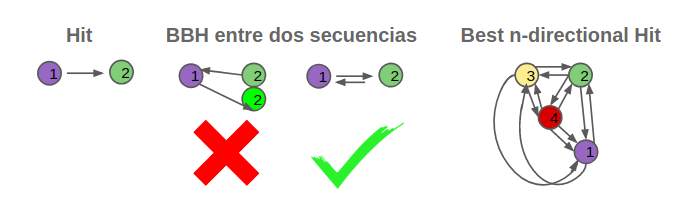
\includegraphics[angle = 0,scale = 1]{chapter1/Best-n-directional.png}
\caption[Best-n-directional]{\normalsize{Best-n-directional}}
\label{fig:Best-n-directional}
\end{figure}

\begin{figure}[h!tbp]
\centering
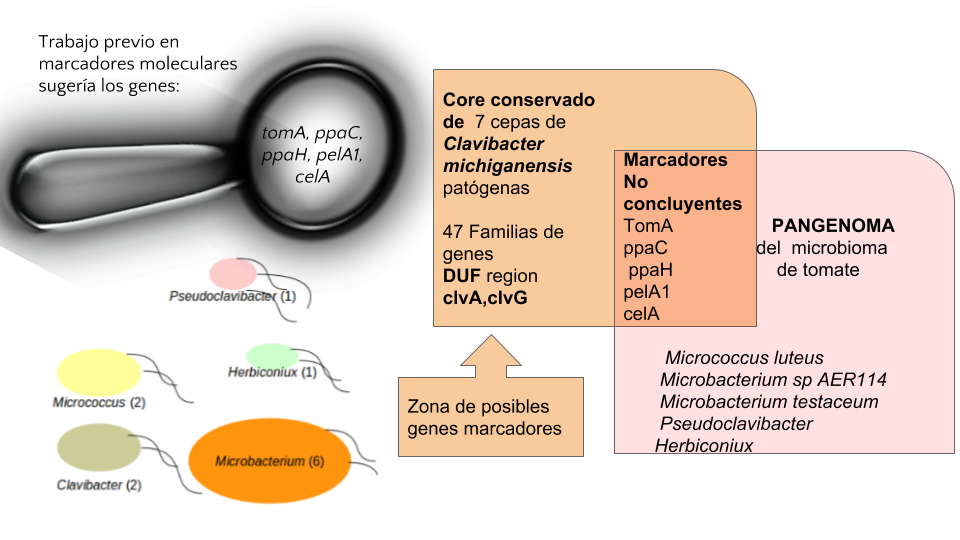
\includegraphics[angle = 0,scale = 1]{chapter1/Marcadores-Clavibacter.png}
\caption[Marcadores-Clavibacter]{\normalsize{Marcadores-Clavibacter}}
\label{fig:Marcadores-Clavibacter}
\end{figure}

\begin{figure}[h!tbp]
\centering
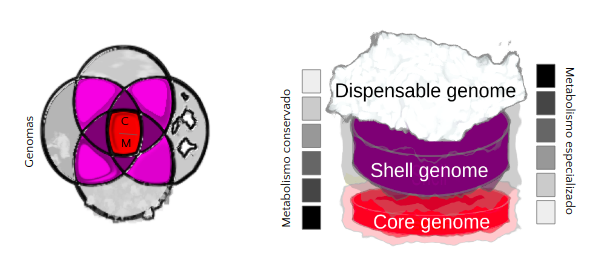
\includegraphics[angle = 0,scale = 1]{chapter1/Metabolismo-Pangenoma.png}
\caption[Metabolismo-Pangenoma]{\normalsize{Metabolismo-Pangenoma}}
\label{fig:Metabolismo-Pangenoma}
\end{figure}

\subsection{Otras aplicaciones de
Orthocore}\label{otras-aplicaciones-de-orthocore}

\subsection{Orthocores resolvió la filogenia de Actinomyces, ayudando a
encontrar perfiles de promiscuidad en
PriA}\label{orthocores-resolvio-la-filogenia-de-actinomyces-ayudando-a-encontrar-perfiles-de-promiscuidad-en-pria}

Orthocores fue diseñado para resolver el problema de \_\_\_\_\_\_\_\_ La
promiscuidad coocurre con variaciones en el contexto genómico. Orthocres
ayudó a establecer la filogenia de actinomyces.

\subsection{\texorpdfstring{Identificación de genes marcadores de
\emph{Clavibacter
michiganensis}}{Identificación de genes marcadores de Clavibacter michiganensis}}\label{identificacion-de-genes-marcadores-de-clavibacter-michiganensis}

Micrococcales es un orden de Actinobacteria que contiene a
\emph{Clavibacter}, \emph{Micrococcus} y \emph{Microbacterium}, entre
otros. Clavibacter es un género que puede causar enfermedades en
plantas. En particular la especie Clavibacter michiganensis es una
bacteria causante de la enfermedad del cancer del tomate. Clavibacter ha
sido frecuentemente aislada en compañía de otros microccocales
morfológicamente parecidos, por lo que una prueba de diagnóstico se
hacía necesaria. de y TomA clvF {[}@yasuhara-bell\_genes\_2014{]}

\begin{figure}[h!tbp]
\centering
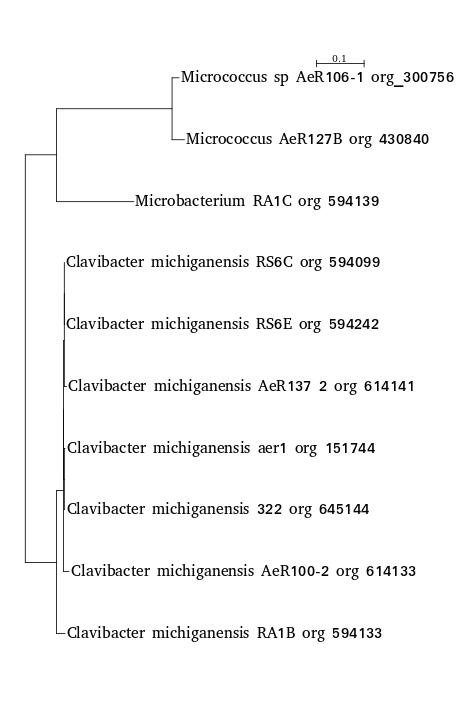
\includegraphics[angle = 0,scale = 1]{chapter1/ArbolOrthocore.png}
\caption[ArbolOrthocore]{\normalsize{ArbolOrthocore}}
\label{fig:ArbolOrthocore}
\end{figure}

\begin{Shaded}
\begin{Highlighting}[]
\NormalTok{table <-}\StringTok{ }\KeywordTok{read.csv}\NormalTok{(}\StringTok{"chapter1/MicrobiomaMetadata.csv"}\NormalTok{, }\DataTypeTok{row.names =} \DecValTok{1}\NormalTok{,}\DataTypeTok{sep=}\StringTok{"}\CharTok{\textbackslash{}t}\StringTok{"}\NormalTok{)}
\KeywordTok{kable}\NormalTok{(table,  }\DataTypeTok{caption =} \StringTok{"Ejemplo de Microbioma }\CharTok{\textbackslash{}\textbackslash{}}\StringTok{label\{tab:Ejemplo de Microbioma\}"}\NormalTok{,}\DataTypeTok{caption.short =} \StringTok{"Microbioma de tomate "}\NormalTok{)}
\end{Highlighting}
\end{Shaded}

\begin{longtable}[]{@{}l@{}}
\caption{Ejemplo de Microbioma
\label{tab:Ejemplo de Microbioma}}\tabularnewline
\toprule
\begin{minipage}[t]{0.97\columnwidth}\raggedright\strut
322,Cmm,Desconocido,Desconocido,2005,Desconocido,Desconocido,Desconocido,Desconocido,Desconocido,6666666.374469\strut
\end{minipage}\tabularnewline
\begin{minipage}[t]{0.97\columnwidth}\raggedright\strut
AER1,Cmm,Agricola el
Rosal,IAT,2010,Enferma,Komeett,desconocido,Monsanto,Plantfort,6666666.6854\strut
\end{minipage}\tabularnewline
\begin{minipage}[t]{0.97\columnwidth}\raggedright\strut
AER1002,Cmm,Agricola el
Rosal,IAT,2013,Enferma,Torero,Multifort,Monsanto,Plantfort,33013.175\strut
\end{minipage}\tabularnewline
\begin{minipage}[t]{0.97\columnwidth}\raggedright\strut
AeR106-1,Micrococcus,Agricola el
Rosal,IAT,2014,Enferma,komeett,desconocido,Monsanto,Plantfort,6666666.155597\strut
\end{minipage}\tabularnewline
\begin{minipage}[t]{0.97\columnwidth}\raggedright\strut
AeR1272,Micrococcus,Agricola el
Rosal,IAT,2015,Enferma,Bigdena,desconocido,Syngenta,Plantfort,6666666.235531\strut
\end{minipage}\tabularnewline
\begin{minipage}[t]{0.97\columnwidth}\raggedright\strut
AER1372,Cmm,Rancho Cipres,IAT,2016,Enferma,Pai Pai,Multifort,enza
zaden,Plantfort,33013.181\strut
\end{minipage}\tabularnewline
\begin{minipage}[t]{0.97\columnwidth}\raggedright\strut
RA1C,Microbacterium,Ninguno,CA,2017,Asintomatica,Silvestre,Ninguno,Ninguno,Ninguno,2.1422\strut
\end{minipage}\tabularnewline
\begin{minipage}[t]{0.97\columnwidth}\raggedright\strut
RS6C,Cmm,Red Sun Farms SMA,Alta tecnologi­a,2018,Marchitez en hojas
tallos amarillos,Komeett,Kaisen,Monsanto,Plantfort,2.1418\strut
\end{minipage}\tabularnewline
\begin{minipage}[t]{0.97\columnwidth}\raggedright\strut
RS6E,Cmm,Red Sun Farms SMA,Alta tecnologÃia,2018,Marchitez en hojas
tallos amarillos,Komeett,Kaisen,Monsanto,Plantfort,2.1425\strut
\end{minipage}\tabularnewline
\begin{minipage}[t]{0.97\columnwidth}\raggedright\strut
RA1B,Clavibacter,Ninguno,CA,2017,Asintomática,Silvestre,Ninguno,Ninguno,Ninguno,2.1421\strut
\end{minipage}\tabularnewline
\bottomrule
\end{longtable}

Había que estandarizar la anotación genpomica, para ello se utilizó la
plataforma myRAST\\
\url{https://github.com/nselem/myrast}\\
\#\#\# Clavisual: Identificación de genes marcadores a un cierto
porcentaje de grupos seleccionados

\begin{figure}[h!tbp]
\centering
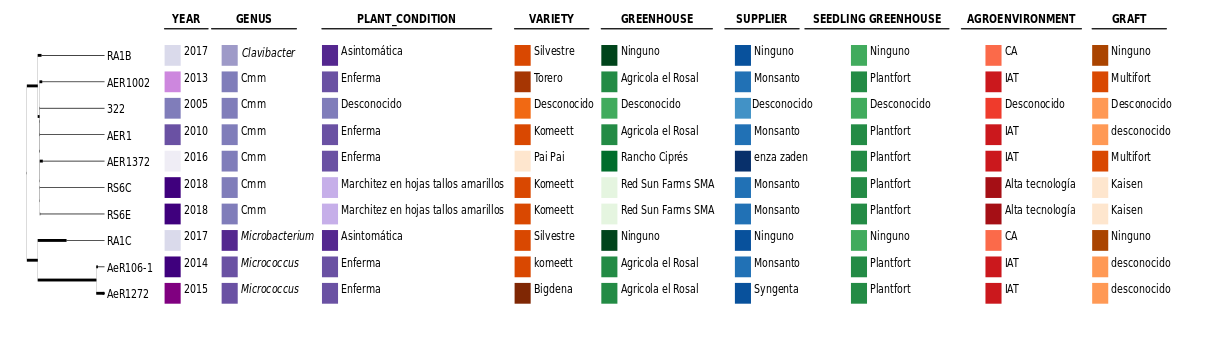
\includegraphics[angle = 0,scale = 1]{chapter1/ArbolClavisual.png}
\caption[ArbolClavisual]{\normalsize{ArbolClavisual}}
\label{fig:ArbolClavisual}
\end{figure}

La idea de que orthocore puede ser usado para obtener los genes
marcadores de un grupo taxonómico frente a otro fue generalizada en el
backend del software Clavisual. Ya se ha explicado previamente que el
core puede salir vacío por diversas razones, entre ellas baja calidad de
los genomas, genomas provenientes de organismos muy divergentes o bien
razones biológicas un core no convergente. Así pues, es posible que si
sólo se utiliza el core no se obtengan marcadores. Pero el core puede
relajarse de varias maneras una de ellas es el Pseudocore, como el core
pero con un genoma de referencia, y a otra es establecer un porcentaje
de presencia /ausencia de interés. El pseudocore consiste en
\_\_\_\_\_\_\_\_ y la metodología está depositada en github en el
repositorio\_\_\_\_\_\_\_\_\_. Los porcentajes de genomas son diferentes
porque al no bastar los best bidireccional hits conservados, todo el
pangenoma es decir todos los genes contenidos en los genomas del grupo
de interés necesitan ser clasificados por familias, para de ahi obtener
las familias que tienen presencia en un porcentaje \%p y ausencia en un
porcentaje a\% del grupo externo. Estos perfiles fueron desarrollados
para Clavisual utilizando FasthOrtho para clasificar las familias y de
ahi obtener los grupos. Con ellos se consiguieron marcadores para
Kutobacterium. Porque qué pasa

El blast del orthocore fue optimizado cambiando hacer un blast todos
contra todos por archivos genómicos individuales
genomai\_vs\_genomaj.blast y luego concatenando estos blasts

\subsection{\texorpdfstring{\emph{Salmonella}}{Salmonella}}\label{salmonella}

Orthocores fue usado aqui para reconstruir filogenias de genomas de
\emph{Salmonella} y como parte del CORASON el algoritmo que sirve para
organizar filogenéticamente variantes de clusters ya sea biosintéticos,
islas de patogenicidad, operones o cualquier región paricalmente
sinténica de un genoma bacteriano centrada en un gen.

\subsection{Relación entre genes marcadores, Orthocores y la
promiscuidad
enzimática.}\label{relacion-entre-genes-marcadores-orthocores-y-la-promiscuidad-enzimatica.}

Finalmente, al aplicar Orthocore para detectar genes marcadores se
vuelve indirectamente reclutamientos al metabolismo especializado, cómo,
pues porque dentro de los marcadores hay productos naturales como la
clavidicina. Hay vemos que clvABCDEF participan en metabolismo
secundario, las enzimas de metabolismo central de este cluster pueden
presentar cierta promiscuidad.

\begin{figure}[h!tbp]
\centering
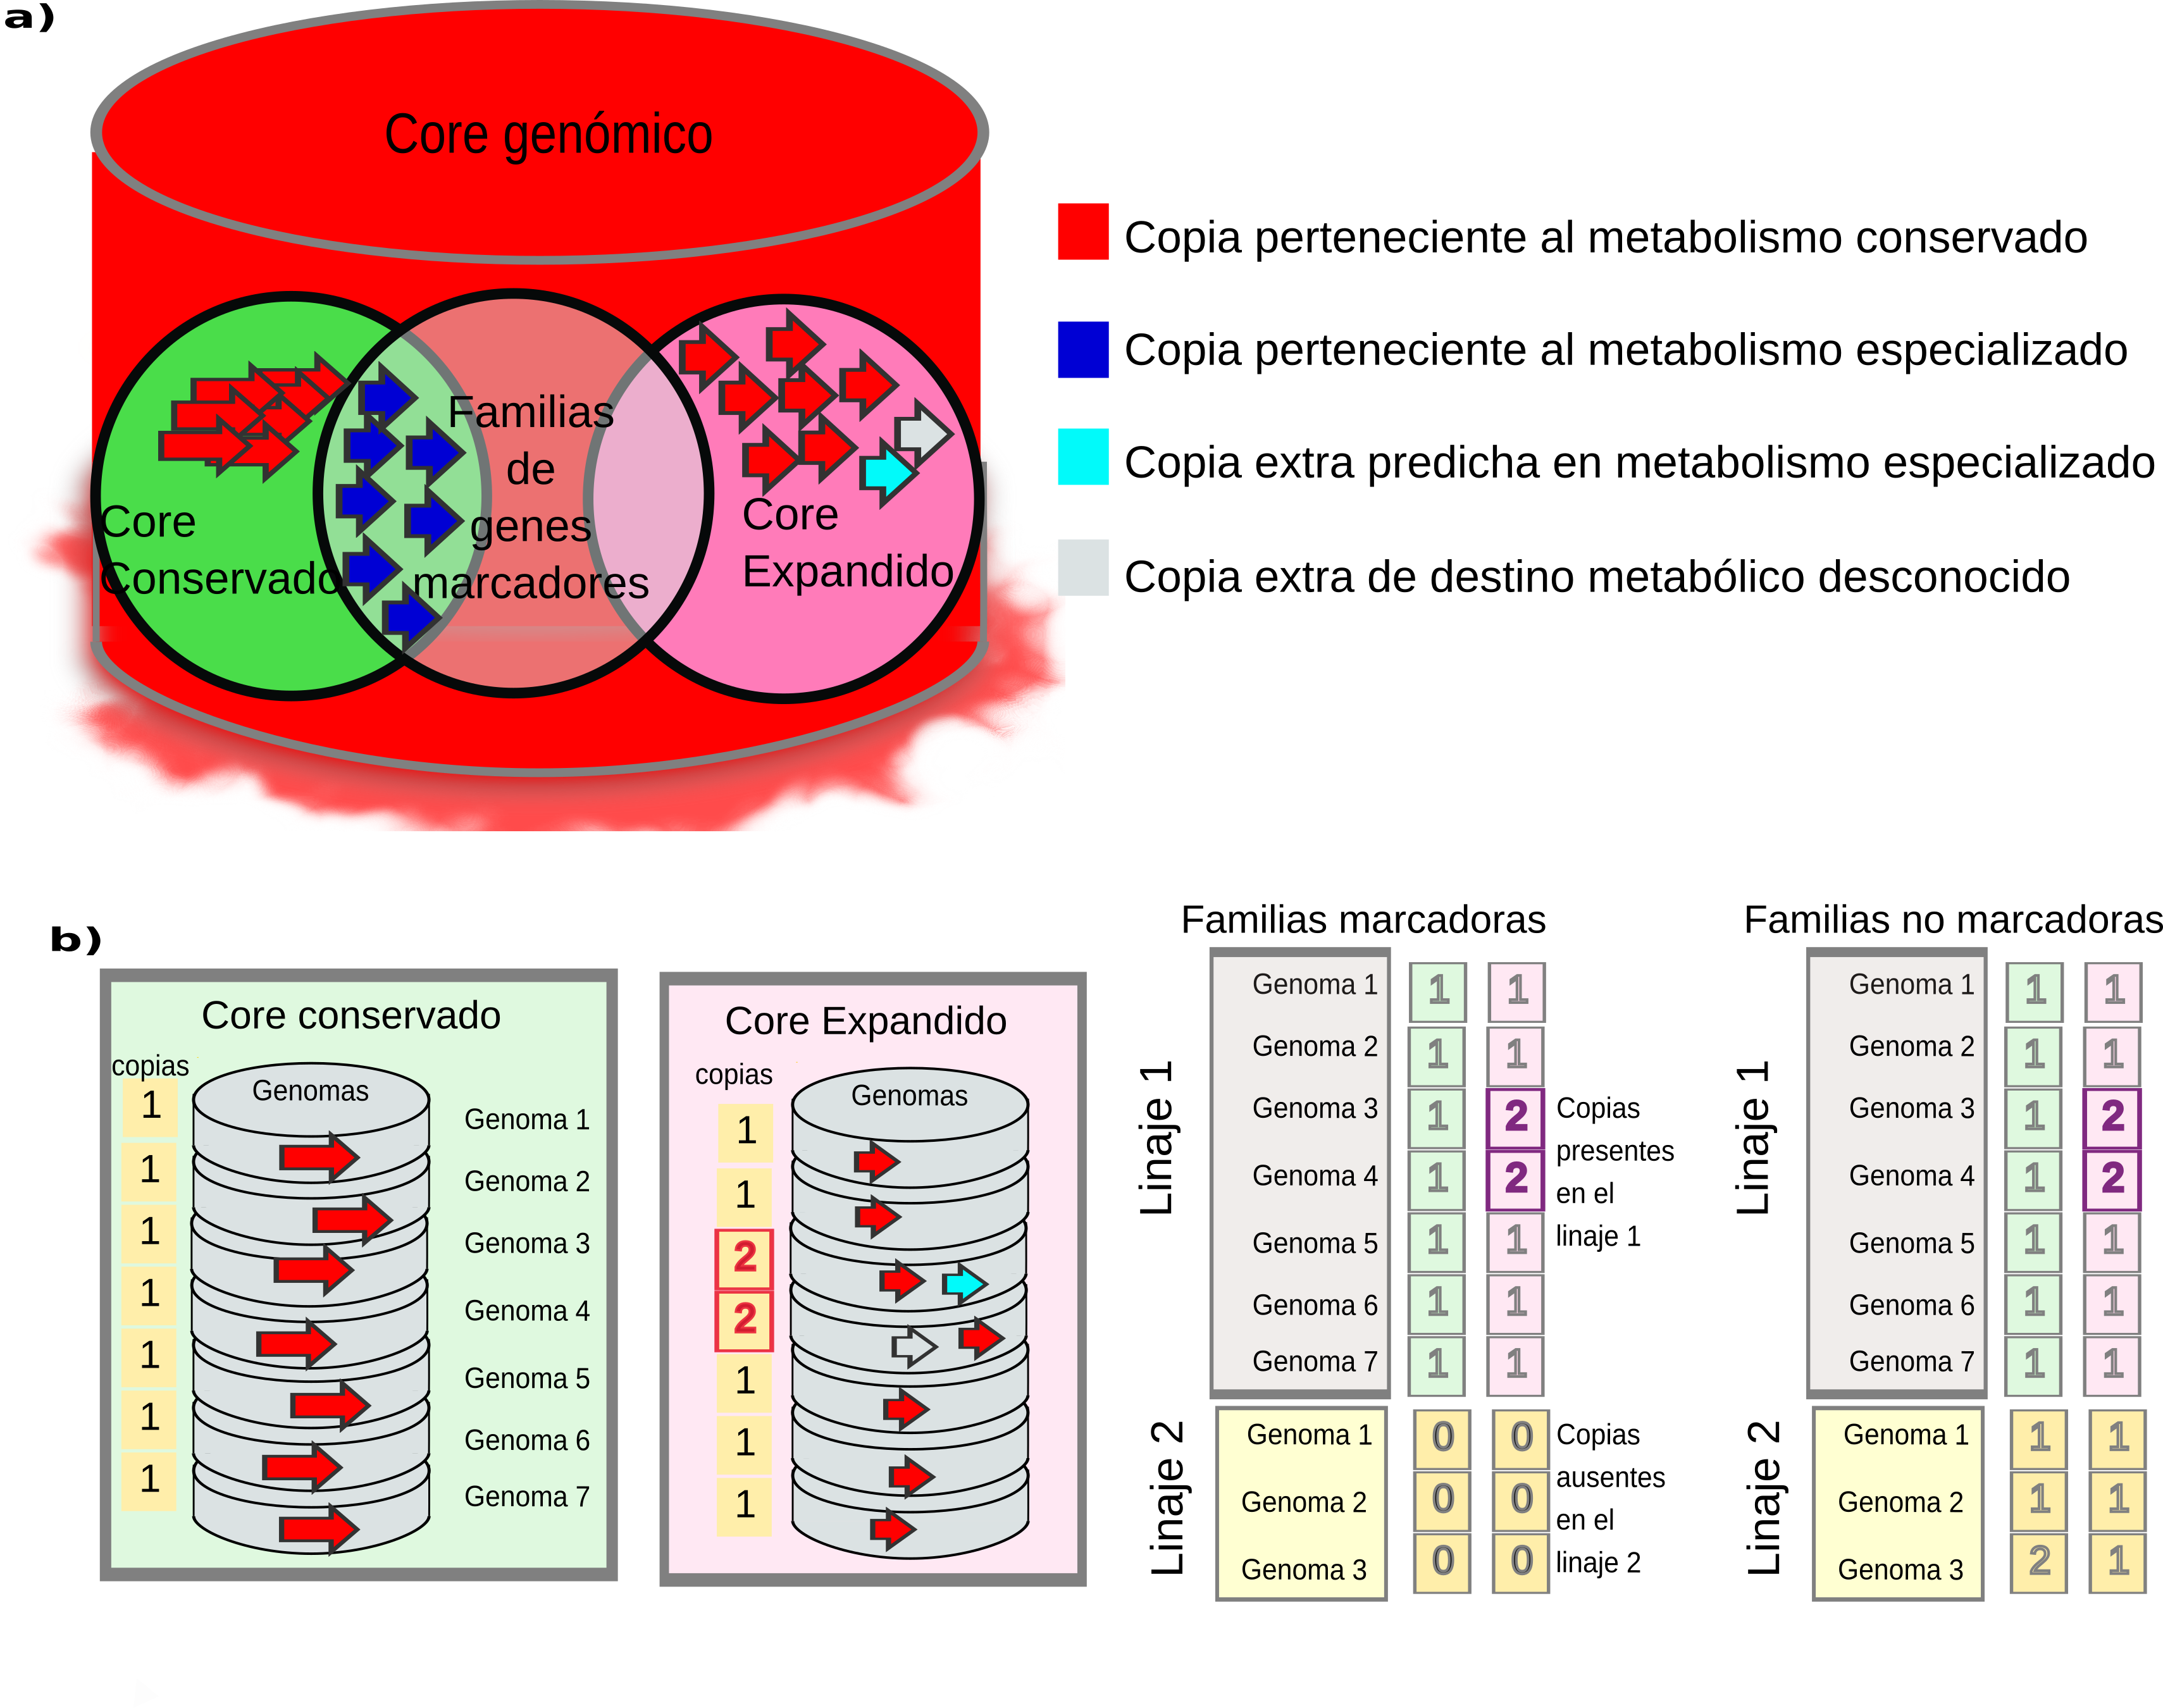
\includegraphics[angle = 0,scale = 1]{chapter1/CoreMarcadores.png}
\caption[CoreMarcadores]{\normalsize{CoreMarcadores}}
\label{fig:CoreMarcadores}
\end{figure}

\begin{Shaded}
\begin{Highlighting}[]
\CommentTok{# Example 1}
\CommentTok{# make a very simple plot}
\NormalTok{x <-}\StringTok{ }\KeywordTok{c}\NormalTok{(}\DecValTok{2}\NormalTok{,}\DecValTok{3}\NormalTok{,}\DecValTok{4}\NormalTok{,}\DecValTok{5}\NormalTok{,}\DecValTok{6}\NormalTok{,}\DecValTok{7}\NormalTok{,}\DecValTok{8}\NormalTok{,}\DecValTok{9}\NormalTok{,}\DecValTok{10}\NormalTok{)}
\NormalTok{y <-}\StringTok{ }\KeywordTok{c}\NormalTok{(}\DecValTok{2684}\NormalTok{,}\DecValTok{2504}\NormalTok{,}\DecValTok{2161}\NormalTok{,}\DecValTok{1867}\NormalTok{,}\DecValTok{1613}\NormalTok{,}\DecValTok{1217}\NormalTok{,}\DecValTok{745}\NormalTok{,}\DecValTok{432}\NormalTok{,}\DecValTok{320}\NormalTok{)}
 \KeywordTok{plot}\NormalTok{(x,y, }\DataTypeTok{xlab=}\StringTok{"Número de genomas "}\NormalTok{, }\DataTypeTok{ylab=}\StringTok{"Número de Genes en el Core genome"}\NormalTok{, }\DataTypeTok{main=}\StringTok{"Core Genome de organismos del Microbioma del tomate"}\NormalTok{, }\DataTypeTok{ylim=}\KeywordTok{c}\NormalTok{(}\DecValTok{0}\NormalTok{,}\DecValTok{4000}\NormalTok{), }\DataTypeTok{xlim=}\KeywordTok{c}\NormalTok{(}\DecValTok{0}\NormalTok{,}\DecValTok{12}\NormalTok{), }\DataTypeTok{pch=}\DecValTok{15}\NormalTok{, }\DataTypeTok{col=}\StringTok{"blue"}\NormalTok{) }
\end{Highlighting}
\end{Shaded}

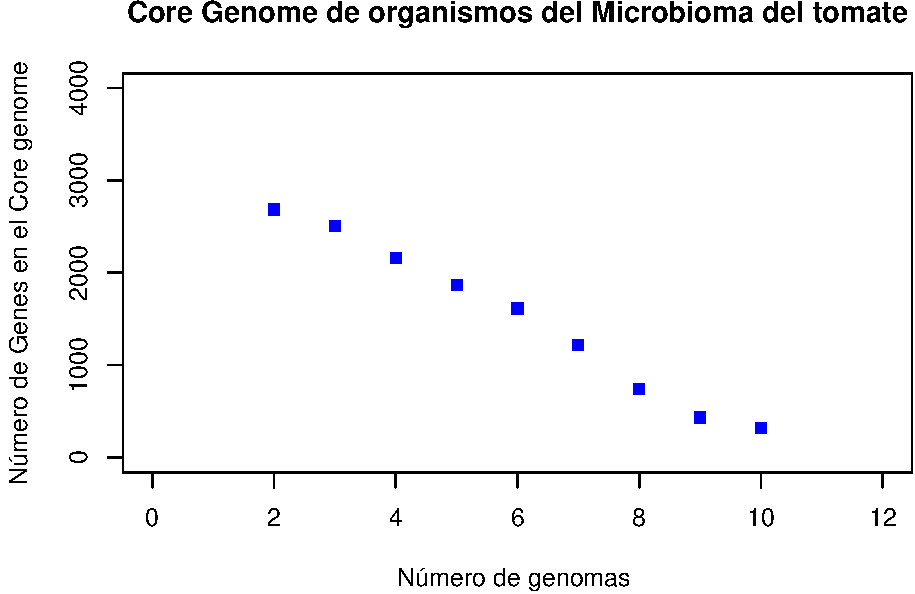
\includegraphics{chap1_files/figure-latex/unnamed-chunk-1-1.pdf}

Lo relevante para la promiscuidad son los procesos de divergencia, por
ello en el siguiente capítulo analizamos encontrar el origin y destino
metabolico, de copias extras de familias enzimáticas. Orthocore está
disponible \url{https://github.com/nselem/orthocore/wiki}


\end{document}
